\documentclass[conference]{IEEEtran}

\usepackage[utf8]{inputenc}
\usepackage[T1]{fontenc}
\usepackage{CJKutf8}
\usepackage{amsmath,amssymb}
\usepackage{graphicx}
\usepackage{booktabs}
\usepackage{multirow}
\usepackage{url}
\usepackage{hyperref}
\usepackage{xcolor}
\usepackage{caption}
\usepackage{subcaption}
\usepackage{array}

\newcolumntype{C}[1]{>{\centering\arraybackslash}p{#1}}

\begin{document}

\title{OrgBench: How Information Flow Design Patterns\\Affect Collective Decision Quality\\in LLM Multi-Agent Systems}

\author{
\IEEEauthorblockN{Wataru Shinoda}
\IEEEauthorblockA{
% Affiliation here
}
}

\maketitle

\begin{abstract}
Large Language Model (LLM) multi-agent systems increasingly adopt organizational metaphors---hierarchies, review protocols, and communication topologies---yet the impact of these \emph{information flow design patterns} on output quality remains poorly understood.
We present \textbf{OrgBench}, a benchmark framework that systematically varies five design dimensions (agent count, hierarchy depth, communication topology, review protocol, and model homogeneity) across 11 configurations, evaluated on business proposal generation tasks.
Through 275 experimental runs with LLM-as-Judge evaluation (550 assessments across 6 quality dimensions), we find that:
(1)~multi-agent configurations significantly outperform single-agent baselines across all dimensions (Cohen's $d = 1.23$--$1.81$);
(2)~shallow hierarchies consistently outperform deep ones ($\Delta = 0.38$--$0.46$);
(3)~mesh communication topology yields marginal gains over hub-and-spoke;
(4)~review protocols improve quality modestly ($\Delta = 0.24$);
and (5)~model quality matters more than organizational structure when models are homogeneous.
All configurations exhibit large effect sizes ($\eta^2 = 0.12$--$0.45$), indicating that information flow design is a first-order concern in multi-agent system engineering.
Our framework and complete experimental artifacts are publicly available for reproducibility.
\end{abstract}

\begin{IEEEkeywords}
Multi-agent systems, Large language models, Information flow, Organizational design, Benchmark
\end{IEEEkeywords}

% ============================================================
\section{Introduction}
\label{sec:intro}
% ============================================================

The rapid proliferation of Large Language Model (LLM)-based multi-agent systems has led to a variety of organizational designs---from simple single-agent pipelines to complex hierarchical structures with specialized roles, review protocols, and diverse communication topologies~\cite{guo2024largelanguagemodelbased, wang2024survey}.
Systems such as ChatDev~\cite{qian2024chatdev}, MetaGPT~\cite{hong2023metagpt}, and AutoGen~\cite{wu2023autogen} implicitly embed assumptions about how information should flow between agents, yet these design choices are rarely evaluated systematically.

A fundamental question remains unanswered: \emph{Do information flow design patterns---hierarchy depth, communication topology, review protocols, and model composition---meaningfully affect the quality of collective outputs?}

This question is critical for practitioners designing multi-agent systems, as the design space is vast and the cost implications are significant.
A deep hierarchy with review protocols requires more LLM calls (and thus higher cost) than a flat structure, but whether this additional cost translates to better outputs is unclear.

We address this gap with \textbf{OrgBench}, a controlled benchmark framework that isolates five key design dimensions through 11 carefully constructed configurations.
Our approach draws on organizational theory~\cite{mintzberg1979structuring, galbraith1974designing} to structure the design space, treating multi-agent systems as information-processing organizations.

Our contributions are:
\begin{enumerate}
    \item A \textbf{systematic taxonomy} of information flow design patterns for LLM multi-agent systems, grounded in organizational theory.
    \item The \textbf{OrgBench framework}, enabling controlled comparison of organizational designs with automated evaluation.
    \item \textbf{Empirical evidence} from 275 runs and 550 evaluations demonstrating that information flow design significantly affects output quality, with large effect sizes across all quality dimensions.
    \item \textbf{Actionable guidelines} for practitioners: prefer shallow hierarchies, include review protocols, and invest in model quality over organizational complexity.
\end{enumerate}

% ============================================================
\section{Related Work}
\label{sec:related}
% ============================================================

\subsection{LLM Multi-Agent Frameworks}

Recent work has explored various architectures for LLM multi-agent collaboration.
ChatDev~\cite{qian2024chatdev} implements a waterfall software development process with specialized agents (CEO, CTO, programmer, tester).
MetaGPT~\cite{hong2023metagpt} introduces Standardized Operating Procedures (SOPs) to coordinate agents, reducing hallucination through structured communication.
AutoGen~\cite{wu2023autogen} provides a flexible framework for multi-agent conversations with customizable interaction patterns.
CAMEL~\cite{li2023camel} explores role-playing between agents for cooperative task solving.

While these systems demonstrate the potential of multi-agent collaboration, they typically evaluate a single organizational design rather than systematically comparing alternatives.

\subsection{Organizational Design in Multi-Agent Systems}

The connection between organizational theory and multi-agent systems has a long history in the MAS community~\cite{horling2004survey}.
Classical organizational theory identifies key structural variables including hierarchy, specialization, and communication patterns~\cite{mintzberg1979structuring}.
Galbraith's information processing view~\cite{galbraith1974designing} frames organizations as information-processing systems, directly applicable to LLM agent architectures.

Recent work has begun exploring organizational structures for LLM agents.
AgentVerse~\cite{chen2023agentverse} investigates group dynamics, while DyLAN~\cite{liu2023dynamic} proposes dynamic agent networks.
However, systematic controlled experiments isolating specific design dimensions remain scarce.

\subsection{LLM-as-Judge Evaluation}

The use of LLMs as evaluators has gained acceptance as a scalable alternative to human evaluation~\cite{zheng2023judging}.
Studies show high correlation between LLM judges and human annotators for structured evaluation tasks~\cite{liu2023geval}.
We adopt this approach with dual independent evaluations per output to improve reliability.

% ============================================================
\section{Experimental Design}
\label{sec:design}
% ============================================================

\subsection{Design Philosophy}

We adopt a \emph{direct orthogonal sampling} approach, where each configuration varies one or two design dimensions from a baseline (anchor) configuration.
This enables attribution of quality differences to specific design choices while keeping the experiment tractable.

\subsection{Design Dimensions}

We identify five key dimensions of information flow design:

\begin{enumerate}
    \item \textbf{Agent Count}: Single agent vs.\ multi-agent (6 agents: CEO, Team Lead, Researcher, Writer, CFO, CDO).
    \item \textbf{Hierarchy Depth}: Flat (CEO $\rightarrow$ all agents) vs.\ deep (CEO $\rightarrow$ TL $\rightarrow$ specialists).
    \item \textbf{Communication Topology}: Hub-and-spoke (through coordinator) vs.\ mesh (peer-to-peer context sharing).
    \item \textbf{Review Protocol}: Presence/absence of CFO and CDO review gates before final output.
    \item \textbf{Model Homogeneity}: Heterogeneous (role-optimized model assignment) vs.\ homogeneous (single model for all agents).
\end{enumerate}

\subsection{Configurations}
\label{subsec:configs}

Table~\ref{tab:configs} summarizes the 11 configurations.
The \textit{anchor} configuration serves as the baseline: deep hierarchy, hub communication, review enabled, heterogeneous models.
Each other configuration differs from the anchor in one or two dimensions.

\begin{table}[t]
\centering
\caption{Experimental configurations. Each varies one or two dimensions from the anchor baseline.}
\label{tab:configs}
\small
\begin{tabular}{lcccc}
\toprule
\textbf{Config} & \textbf{Depth} & \textbf{Comm.} & \textbf{Review} & \textbf{Models} \\
\midrule
anchor & deep & hub & \checkmark & hetero \\
flat\_hub & flat & hub & \checkmark & hetero \\
flat\_mesh & flat & mesh & \checkmark & hetero \\
matrix\_hub & deep & hub+mesh & \checkmark & hetero \\
deep\_mesh & deep & mesh & \checkmark & hetero \\
deep\_finance & deep & hub & CFO+ & hetero \\
deep\_tech & deep & hub & CDO+ & hetero \\
deep\_noreview & deep & hub & $\times$ & hetero \\
homo\_haiku & deep & hub & \checkmark & all-Haiku \\
homo\_gpt & deep & hub & \checkmark & all-GPT \\
single\_agent & --- & --- & $\times$ & Haiku \\
\bottomrule
\end{tabular}
\end{table}

\subsection{Task and Themes}

We use \textbf{business proposal generation} as the evaluation task, requiring integration of market research, financial analysis, and technical assessment---naturally suited to multi-agent collaboration.

Five diverse themes are used:
(1)~AI-powered accounting automation for SMEs,
(2)~AI legal document review,
(3)~government chatbot services,
(4)~elderly fitness technology,
and (5)~AI insurance underwriting.

\subsection{Model Assignment}

For heterogeneous configurations, models are assigned by role:
CEO uses Claude Haiku 4.5 (decision-making),
operational agents (TL, Writer, CFO, CDO) use GPT-4o-mini (cost-efficient execution),
and Researcher uses Gemini 2.5 Flash (web search integration).
Homogeneous configurations use a single model for all roles.

\subsection{Evaluation: LLM-as-Judge}

Each output is evaluated independently twice by Gemini 2.5 Flash across six quality dimensions on a 1--5 Likert scale:

\begin{itemize}
    \item \textbf{Feasibility}: Realism of implementation plan
    \item \textbf{Novelty}: Originality and differentiation
    \item \textbf{Market Insight}: Depth of market/competitive analysis
    \item \textbf{Financial Rigor}: Quality of financial projections
    \item \textbf{Technical Depth}: Sophistication of technical design
    \item \textbf{Overall Quality}: Holistic assessment
\end{itemize}

A detailed rubric with anchoring examples guides the evaluation (see supplementary materials).

\subsection{Experimental Protocol}

Each configuration--theme pair is replicated 5 times ($N = 11 \times 5 \times 5 = 275$ runs).
Each output receives 2 independent judge evaluations ($550$ total assessments).
Temperature is set to 0.7 for generation and 0.3 for evaluation.
All runs use a 600-second timeout.

% ============================================================
\section{Results}
\label{sec:results}
% ============================================================

\subsection{Overall Quality Rankings}

Fig.~\ref{fig:overall} presents the overall quality scores with standard deviations for all 11 configurations.
Table~\ref{tab:scores} provides the full breakdown across all quality dimensions.
The flat\_mesh configuration achieves the highest overall quality (3.30), followed by flat\_hub and homo\_haiku (both 3.22).
Single\_agent ranks last at 1.82.

\begin{figure}[t]
\centering
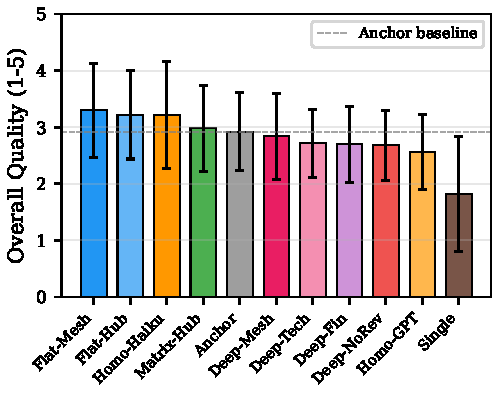
\includegraphics[width=\columnwidth]{figures/fig1_overall_quality.pdf}
\caption{Overall quality scores by configuration (mean $\pm$ SD). Dashed line indicates the anchor baseline. Multi-agent configurations consistently outperform the single-agent baseline.}
\label{fig:overall}
\end{figure}

\begin{table}[t]
\centering
\caption{Mean quality scores by configuration (sorted by overall quality). $n = 50$ per configuration (5 themes $\times$ 5 reps $\times$ 2 judge runs).}
\label{tab:scores}
\small
\begin{tabular}{lcccccc}
\toprule
\textbf{Config} & \textbf{Feas.} & \textbf{Nov.} & \textbf{Mkt.} & \textbf{Fin.} & \textbf{Tech.} & \textbf{OQ} \\
\midrule
flat\_mesh    & 3.32 & 4.14 & 4.84 & 2.90 & 2.58 & \textbf{3.30} \\
flat\_hub     & 3.20 & 4.12 & 4.98 & 2.66 & 3.16 & \textbf{3.22} \\
homo\_haiku   & 3.62 & 3.84 & 4.34 & 3.26 & 2.76 & \textbf{3.22} \\
matrix\_hub   & 3.20 & 4.04 & 5.00 & 2.50 & 2.52 & 2.98 \\
anchor        & 3.26 & 3.76 & 4.96 & 2.58 & 2.42 & 2.92 \\
deep\_mesh    & 3.16 & 3.84 & 4.90 & 2.46 & 2.38 & 2.84 \\
deep\_tech    & 3.14 & 4.04 & 4.96 & 2.26 & 2.28 & 2.72 \\
deep\_finance & 3.12 & 3.88 & 4.96 & 2.60 & 1.80 & 2.70 \\
deep\_noreview& 3.06 & 3.68 & 4.88 & 2.60 & 2.08 & 2.68 \\
homo\_gpt     & 3.32 & 2.54 & 3.58 & 2.74 & 2.52 & 2.56 \\
single\_agent & 2.02 & 2.22 & 2.96 & 1.38 & 1.68 & \textbf{1.82} \\
\bottomrule
\end{tabular}
\end{table}

\subsection{Effect Sizes}

Table~\ref{tab:effects} and Fig.~\ref{fig:effects} report the effect sizes for each quality dimension.
All dimensions show large $\eta^2$ values ($> 0.14$), except technical\_depth which shows a medium effect.
Cohen's $d$ between single-agent and the best multi-agent configuration is consistently large ($> 0.8$) across all dimensions.

\begin{figure}[t]
\centering
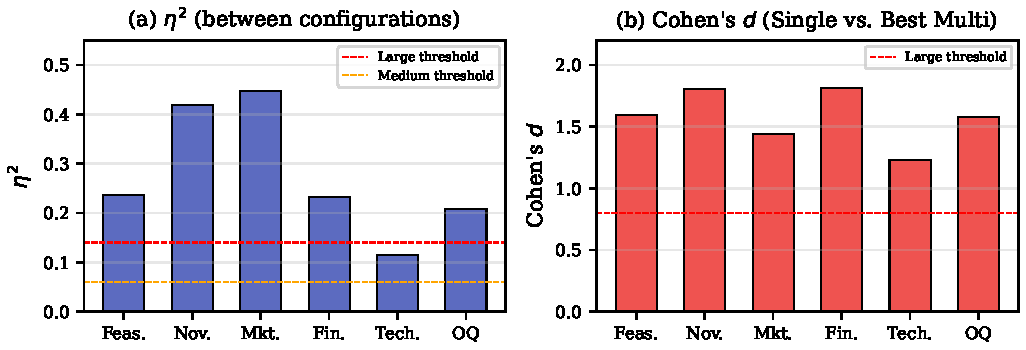
\includegraphics[width=\columnwidth]{figures/fig3_effect_sizes.pdf}
\caption{Effect sizes across quality dimensions. (a)~$\eta^2$ quantifies variance explained by configuration differences. (b)~Cohen's $d$ measures the gap between single-agent and the best multi-agent configuration. Dashed lines indicate conventional thresholds.}
\label{fig:effects}
\end{figure}

\begin{table}[t]
\centering
\caption{Effect sizes across quality dimensions.}
\label{tab:effects}
\begin{tabular}{lccl}
\toprule
\textbf{Dimension} & $\boldsymbol{\eta^2}$ & \textbf{Cohen's} $\boldsymbol{d}$ & \textbf{Size} \\
\midrule
Feasibility      & 0.236 & +1.59 & large \\
Novelty          & 0.418 & +1.81 & large \\
Market Insight   & 0.448 & +1.44 & large \\
Financial Rigor  & 0.233 & +1.81 & large \\
Technical Depth  & 0.116 & +1.23 & med./large \\
Overall Quality  & 0.208 & +1.58 & large \\
\bottomrule
\end{tabular}
\end{table}

\subsection{Quality Profile Analysis}

Fig.~\ref{fig:radar} shows the quality profiles of four representative configurations.
The single-agent baseline (brown) is uniformly inferior, while multi-agent configurations show distinct strengths: Flat-Mesh excels in novelty and market insight, while Homo-Haiku leads in feasibility and financial rigor.
Fig.~\ref{fig:heatmap} provides the complete quality landscape across all configurations and dimensions.

\begin{figure}[t]
\centering
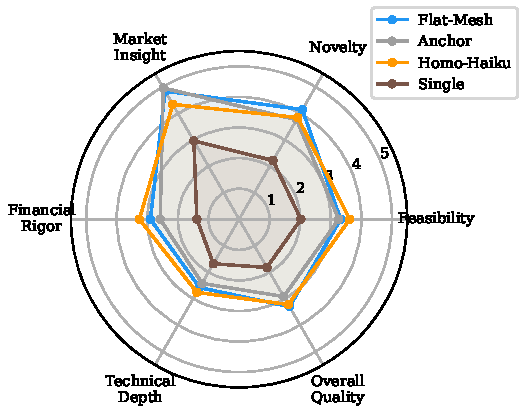
\includegraphics[width=0.85\columnwidth]{figures/fig2_radar.pdf}
\caption{Quality profiles of four representative configurations. Multi-agent systems (Flat-Mesh, Anchor, Homo-Haiku) consistently envelop the single-agent baseline across all dimensions.}
\label{fig:radar}
\end{figure}

\begin{figure}[t]
\centering
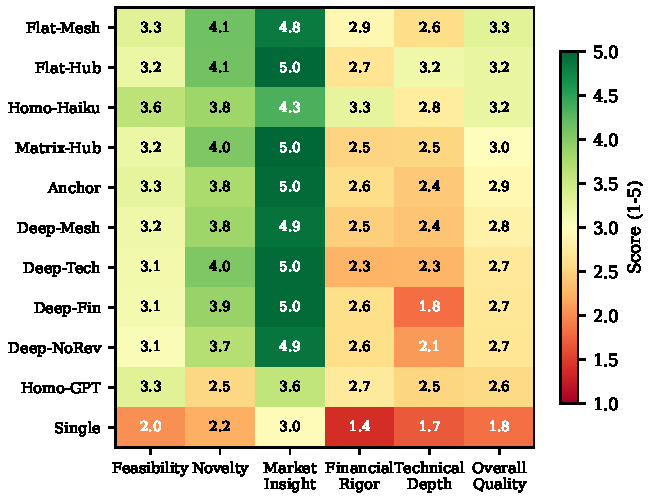
\includegraphics[width=\columnwidth]{figures/fig4_heatmap.pdf}
\caption{Quality heatmap across all configurations and dimensions. Darker green indicates higher scores. The single-agent row (bottom) shows uniformly lower scores.}
\label{fig:heatmap}
\end{figure}

\subsection{Research Question Analysis}

\subsubsection{RQ1: Multi-Agent vs.\ Single Agent}

Multi-agent configurations dramatically outperform the single-agent baseline across all quality dimensions (Table~\ref{tab:effects}).
The best multi-agent configuration (flat\_mesh, OQ $= 3.30$) scores 1.48 points higher than single\_agent (OQ $= 1.82$), with Cohen's $d = 1.58$.
This effect is most pronounced for financial rigor ($d = 1.81$) and novelty ($d = 1.81$), suggesting that specialized agents contribute domain-specific depth that a single generalist agent cannot replicate.

\subsubsection{RQ2: Hierarchy Depth}

Fig.~\ref{fig:pairwise}(a) shows the pairwise comparisons.
Shallow (flat) hierarchies consistently outperform deep ones:
flat\_mesh (3.30) $>$ deep\_mesh (2.84);
flat\_hub (3.22) $>$ anchor (2.92).
The difference ($\Delta = 0.38$--$0.46$) suggests that deep hierarchies introduce information loss through additional mediation layers.
This aligns with information theory: each relay point introduces potential distortion~\cite{galbraith1974designing}.

\subsubsection{RQ3: Communication Topology}

As shown in Fig.~\ref{fig:pairwise}(b), mesh communication shows modest advantages over hub-and-spoke:
flat\_mesh (3.30) $\geq$ flat\_hub (3.22);
deep\_mesh (2.84) $\approx$ anchor (2.92).
The matrix\_hub configuration (2.98), which combines hub and mesh elements, falls between pure topologies.
The effect of topology is smaller than that of hierarchy depth.

\subsubsection{RQ4: Review Protocol}

Fig.~\ref{fig:pairwise}(c) illustrates the review effect.
Review protocols provide a modest quality improvement:
anchor (2.92) $>$ deep\_noreview (2.68), $\Delta = 0.24$.
While the effect is consistent, it is the smallest among the design dimensions studied.
Specialized review emphasis (deep\_finance, deep\_tech) does not improve over the standard review protocol and may even reduce quality in non-emphasized dimensions.

\subsubsection{RQ5: Model Homogeneity}

Fig.~\ref{fig:pairwise}(d) reveals that model quality dominates organizational structure when all agents use the same model:
homo\_haiku (3.22, all Claude Haiku) $\gg$ homo\_gpt (2.56, all GPT-4o-mini).
Notably, homo\_haiku matches the performance of the best heterogeneous configurations despite using a simpler model assignment strategy, though at significantly higher cost (\$3.66 vs.\ \$0.81--\$1.00).

\subsection{Cost-Quality Trade-off}

Fig.~\ref{fig:cost} visualizes the cost-quality trade-off across all configurations.

\begin{figure}[t]
\centering
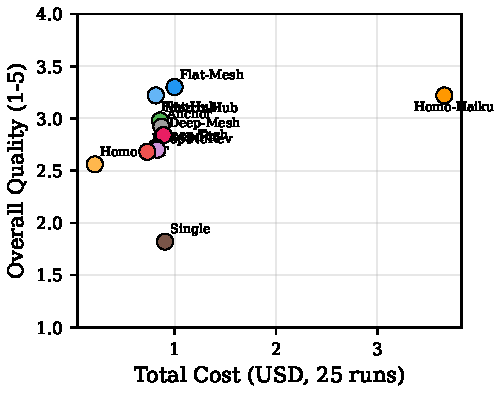
\includegraphics[width=\columnwidth]{figures/fig5_cost_quality.pdf}
\caption{Cost vs.\ quality trade-off. Flat-Hub and Flat-Mesh achieve top-tier quality at moderate cost, while Homo-Haiku achieves similar quality at 4$\times$ the cost. Single-agent costs as much as heterogeneous multi-agent configurations but produces substantially lower quality.}
\label{fig:cost}
\end{figure}

\begin{figure*}[t]
\centering
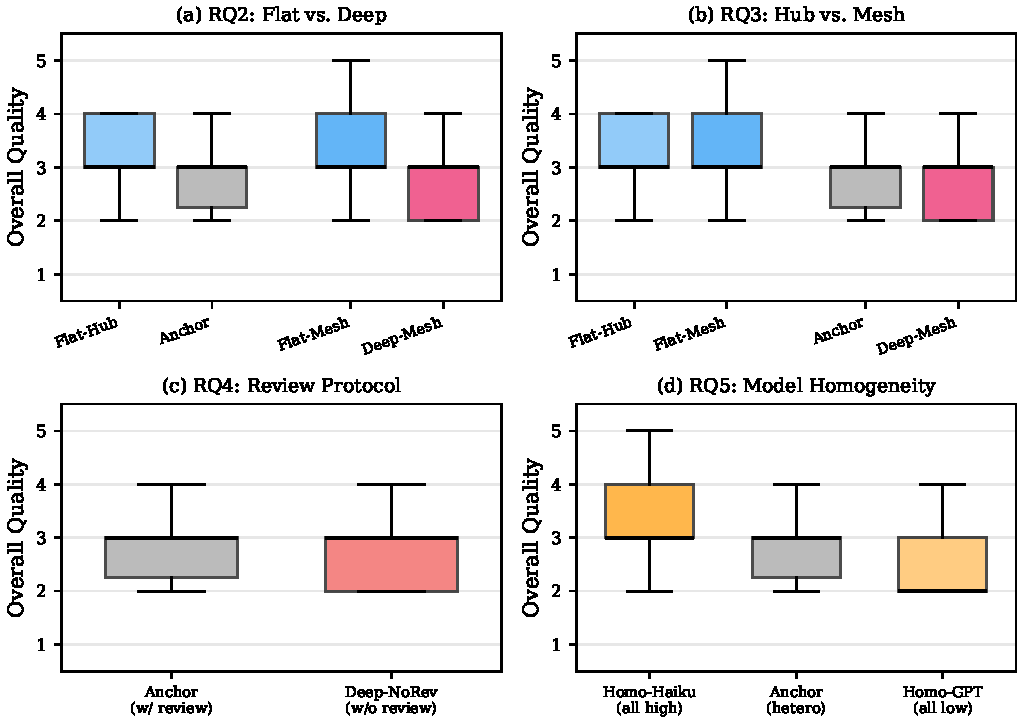
\includegraphics[width=0.95\textwidth]{figures/fig6_pairwise.pdf}
\caption{Pairwise comparisons for each research question (box plots of overall quality). (a)~Flat hierarchies consistently outperform deep ones. (b)~Hub and mesh topologies show similar distributions. (c)~Review protocols provide modest improvement. (d)~High-quality homogeneous models (Homo-Haiku) match heterogeneous configurations.}
\label{fig:pairwise}
\end{figure*}

\begin{table}[t]
\centering
\caption{Cost-quality trade-off per configuration (25 runs each).}
\label{tab:cost}
\small
\begin{tabular}{lccc}
\toprule
\textbf{Config} & \textbf{Cost (\$)} & \textbf{OQ} & \textbf{OQ/\$} \\
\midrule
homo\_gpt     & 0.21 & 2.56 & 12.19 \\
deep\_noreview& 0.73 & 2.68 & 3.67 \\
flat\_hub     & 0.81 & 3.22 & 3.98 \\
flat\_mesh    & 1.00 & 3.30 & 3.30 \\
anchor        & 0.87 & 2.92 & 3.36 \\
homo\_haiku   & 3.66 & 3.22 & 0.88 \\
single\_agent & 0.91 & 1.82 & 2.00 \\
\bottomrule
\end{tabular}
\end{table}

Table~\ref{tab:cost} reveals that \textbf{flat\_hub} achieves the best cost-quality balance: it matches homo\_haiku's quality (3.22) at 22\% of the cost.
Homo\_gpt offers the highest cost efficiency but at lower absolute quality.

% ============================================================
\section{Discussion}
\label{sec:discussion}
% ============================================================

\subsection{Implications for System Design}

Our findings yield several practical guidelines for designing LLM multi-agent systems:

\textbf{Prefer flat hierarchies.}
Deep hierarchies add cost and latency without improving quality.
In information-processing terms, each hierarchical layer acts as a bottleneck that may filter or distort information~\cite{galbraith1974designing}.
Direct access between the coordinator and specialist agents preserves information fidelity.

\textbf{Include review protocols, but keep them lightweight.}
Standard review by domain experts (CFO, CDO) improves quality, but over-emphasizing a single review perspective (deep\_finance, deep\_tech) can be counterproductive.

\textbf{Invest in model quality when budget permits.}
The homo\_haiku result demonstrates that a capable model in a standard organizational structure can match optimized heterogeneous configurations.
However, the 4$\times$ cost premium may not justify this for most applications.

\textbf{Multi-agent is clearly superior to single-agent for complex tasks.}
The large effect sizes ($d > 1.2$) across all dimensions confirm that task decomposition and role specialization provide substantial benefits.

\subsection{Theoretical Implications}

Our results provide empirical support for Galbraith's information processing view~\cite{galbraith1974designing} applied to LLM systems: the capacity to process information (through parallel specialized agents) improves output quality, but excessive mediation layers (deep hierarchies) create information loss.

The finding that flat structures outperform deep ones contrasts with some human organizational literature favoring hierarchical coordination for complex tasks~\cite{mintzberg1979structuring}.
This may reflect a key difference between human and LLM agents: LLMs do not suffer from cognitive overload when processing large contexts, making flat coordination less costly than in human organizations.

\subsection{Limitations}

\textbf{Task scope.}
We evaluate only business proposal generation.
Generalization to coding, creative writing, or scientific tasks requires further study.

\textbf{Judge bias.}
Evaluation relies on a single judge model (Gemini 2.5 Flash).
Cross-model judge validation would strengthen confidence in the results.

\textbf{Model specificity.}
Results are tied to current model capabilities.
As models evolve, the relative advantages of organizational designs may shift.

\textbf{Prompt sensitivity.}
Agent prompts were designed once and not optimized.
Different prompts might alter the ranking of configurations.

% ============================================================
\section{Conclusion}
\label{sec:conclusion}
% ============================================================

We presented OrgBench, a systematic benchmark for evaluating information flow design patterns in LLM multi-agent systems.
Through 275 experimental runs and 550 quality assessments, we demonstrated that organizational design significantly affects output quality with large effect sizes.

Key findings include:
(1)~multi-agent systems substantially outperform single agents;
(2)~flat hierarchies outperform deep ones;
(3)~review protocols provide modest but consistent improvements;
(4)~communication topology has a smaller effect than hierarchy depth;
and (5)~model quality can substitute for organizational complexity when budget permits.

These results establish information flow design as a first-order engineering concern and provide empirically grounded guidelines for practitioners.
Future work includes expanding to additional task domains, cross-model judge validation, and investigating dynamic organizational adaptation.

% ============================================================
% References
% ============================================================

\bibliographystyle{IEEEtran}

\begin{thebibliography}{10}

\bibitem{guo2024largelanguagemodelbased}
T.~Guo, X.~Chen, Y.~Wang, R.~Chang, S.~Pei, N.~V. Chawla, O.~Wiest, and X.~Zhang,
``Large language model based multi-agents: A survey of progress and challenges,''
\emph{arXiv preprint arXiv:2402.01680}, 2024.

\bibitem{wang2024survey}
L.~Wang, C.~Ma, X.~Feng, Z.~Zhang, H.~Yang, J.~Zhang, Z.~Chen, J.~Tang, X.~Chen, Y.~Lin, W.~X. Zhao, Z.~Wei, and J.~Wen,
``A survey on large language model based autonomous agents,''
\emph{Frontiers of Computer Science}, vol.~18, no.~6, 2024.

\bibitem{qian2024chatdev}
C.~Qian, W.~Liu, H.~Liu, N.~Chen, Y.~Dang, J.~Li, C.~Yang, W.~Chen, Y.~Su, X.~Cong, J.~Xu, D.~Li, Z.~Liu, and M.~Sun,
``ChatDev: Communicative agents for software development,''
in \emph{Proc.\ ACL}, 2024.

\bibitem{hong2023metagpt}
S.~Hong, M.~Zhuge, J.~Chen, X.~Zheng, Y.~Cheng, C.~Zhang, J.~Wang, Z.~Wang, S.~K.~S. Yau, Z.~Lin, L.~Zhou, C.~Ran, L.~Xiao, C.~Wu, and J.~Schmidhuber,
``MetaGPT: Meta programming for a multi-agent collaborative framework,''
in \emph{Proc.\ ICLR}, 2024.

\bibitem{wu2023autogen}
Q.~Wu, G.~Bansal, J.~Zhang, Y.~Wu, B.~Li, E.~Zhu, L.~Jiang, X.~Zhang, S.~Zhang, J.~Liu, A.~H. Awadallah, R.~W. White, D.~Burger, and C.~Wang,
``AutoGen: Enabling next-gen LLM applications via multi-agent conversation,''
\emph{arXiv preprint arXiv:2308.08155}, 2023.

\bibitem{li2023camel}
G.~Li, H.~A.~A.~K. Hammoud, H.~Itani, D.~Khizbullin, and B.~Ghanem,
``CAMEL: Communicative agents for `mind' exploration of large language model society,''
in \emph{Proc.\ NeurIPS}, 2023.

\bibitem{horling2004survey}
B.~Horling and V.~Lesser,
``A survey of multi-agent organizational paradigms,''
\emph{The Knowledge Engineering Review}, vol.~19, no.~4, pp.~281--316, 2004.

\bibitem{mintzberg1979structuring}
H.~Mintzberg,
\emph{The Structuring of Organizations}.
Prentice-Hall, 1979.

\bibitem{galbraith1974designing}
J.~R. Galbraith,
``Organization design: An information processing view,''
\emph{Interfaces}, vol.~4, no.~3, pp.~28--36, 1974.

\bibitem{chen2023agentverse}
W.~Chen, Y.~Su, J.~Zuo, C.~Yang, C.~Yuan, C.~Qian, C.~M. Chan, Y.~Qin, Y.~Lu, R.~Xie, Z.~Liu, M.~Sun, and J.~Zhou,
``AgentVerse: Facilitating multi-agent collaboration and exploring emergent behaviors,''
in \emph{Proc.\ ICLR}, 2024.

\bibitem{liu2023dynamic}
Z.~Liu, Y.~Zhang, P.~Li, Y.~Liu, and D.~Yang,
``Dynamic LLM-agent network: An LLM-agent collaboration framework with agent team optimization,''
\emph{arXiv preprint arXiv:2310.02170}, 2023.

\bibitem{zheng2023judging}
L.~Zheng, W.-L. Chiang, Y.~Sheng, S.~Zhuang, Z.~Wu, Y.~Zhuang, Z.~Lin, Z.~Li, D.~Li, E.~P. Xing, H.~Zhang, J.~E. Gonzalez, and I.~Stoica,
``Judging LLM-as-a-judge with MT-Bench and Chatbot Arena,''
in \emph{Proc.\ NeurIPS}, 2023.

\bibitem{liu2023geval}
Y.~Liu, D.~Iter, Y.~Xu, S.~Wang, R.~Xu, and C.~Zhu,
``G-Eval: NLG evaluation using GPT-4 with better human alignment,''
in \emph{Proc.\ EMNLP}, 2023.

\end{thebibliography}

\end{document}
